\chapter{Basic data analysis}
\label{cha:1}
In this chapter details of the dataset are introduced and a basic analysis is performed. This includes assessing missing data, seasonality,  influence of temperature and household data, comparing weekdays and weekends, applying an ARIMA model for forecasting.

% Look at the comments during the meeting 'writing the WTK thesis'.
% Make sure that write every part sufficient substantiated.

\section{Introduction to dataset}
% how the dataset is made up --> use the information of the competition.
The data that is used in this thesis is made available for the \href{https://ieee-dataport.org/competitions/ieee-cis-technical-challenge-energy-prediction-smart-meter-data}{IEEE-CIS technical challenge on energy prediction from smart data}. It consists out of data from smart meters about the 1/2 hour granulated electricity consumption of $3248$ households located in the United Kingdom in the year $2017$. Each smart meter collected thus a total of $17520$ measurements that are performed by the the leading international energy provider, E.ON UK plc. Not all the $3248$ smart meters consist of full data as can be seen in Figure \ref{fig:amountNaN} in appendix \ref{app:A}. It can be clearly seen that there are $12$ steps in the amount of missing values. This is because the available data ranges from one month (only December) to a full year of data. This acknowledges that customers may have joined at different times during the year. Additionally, missing values are introduced due to errors in sending/receiving from smart meters.\\
Next to the electricity consumption of the different households, also information is available about the average, minimum and maximum temperature of the day on the location of the smart meter. This data is available at a daily resolution. Also, through voluntary surveys, incomplete information is collected about $2143$ smart meters. This concerns e.g. dwelling type, number of occupants, number of bedrooms etc. Table \ref{tab:attributes} displays all the attributes in appendix \ref{app:A}.\\

%After substituting the missing values as discussed in \ref{s:missing_data}, all the available weeks are averaged out over all the $270$ smart meters that contain a full year of measurements. The result is given by Figure \ref{fig:averaged_week}. A difference that with belgian load profiles is the consumption peak after midnight. This is due to the higher use of the electric storage heaters used in the UK. These systems store electric energy when the electric tariff is low e.g. overnight and releases the heat when the tariff is high.
%

\section{Preprocessing}

Following steps discuss the preprocessing done on the consumption time-series containing measurements for the entire year. 

\subsection{Missing data} \label{s:missing_data}
As discussed above the consumption dataset contains additionally to the missing months also missing data due to sending/receiving errors of the smart meters. When this happens the data of the whole day is lost. Two methods to impute the missing values are compared. Method one substitutes the missing values of a time-serie by the mean of all the measurements done by the meter. Method two replaces the missing values by the mean consumption value of the same moment on the next and previous day. If the next or previous day is also missing, the closest known day is used. The resulting signals can be seen in Figure \ref{fig:mv_mean} and Figure \ref{fig:mv_s} in appendix \ref{app:A}.\\

In order to ascertain which method of the two performs the best, a reference dataset is needed in order to compare the estimated with the true values of the missing measurements. From the original dataset which contain $ 3248 $ meters it was found that for $ 181 $ meters the month March was given without missing data. These $ 181 $ complete signals of the month March are used as reference dataset. In order to create the test data in each of the $ 181  $ meter signals $ 7 $ random days of the month March were removed and estimated by the earlier two methods. The normalized mean square errors, $ MSE_{AN} $ and $ MSE_{mean} $ given by $ \sum_{i=1}^{D} e_i^2  $ and normalized by $ MSE_{mean} $ are given in Figure \ref{fig:mv_result}.

\begin{figure}[h!]
	\centering
	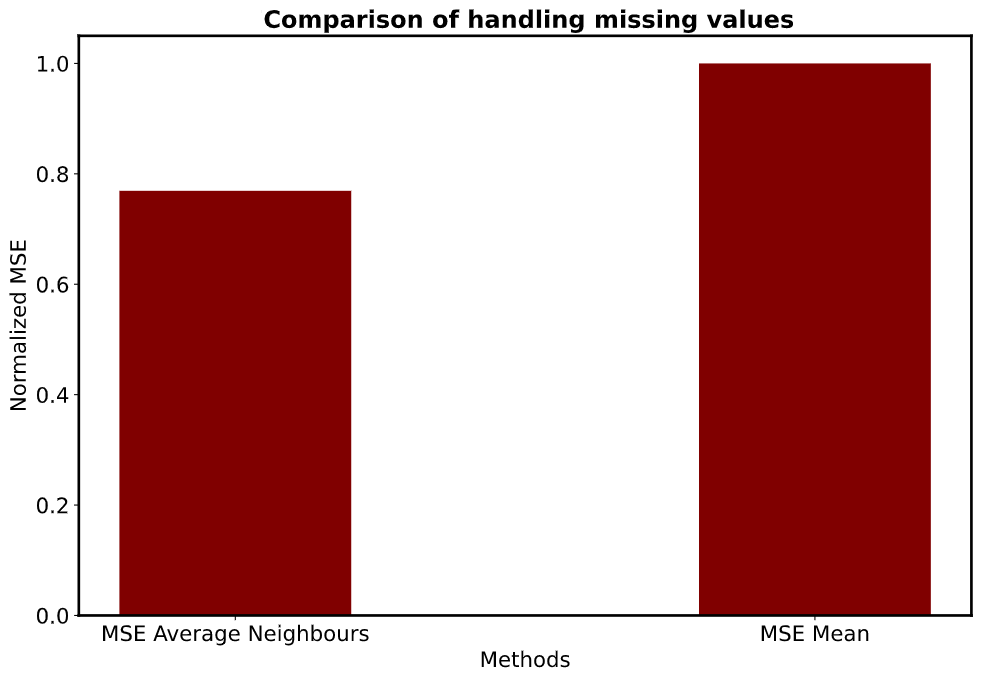
\includegraphics[width=0.8\textwidth]{mv_result.png}
	\caption{Resulting month of March after substitution of the missing values by the mean value of the measurements. }
	\label{fig:mv_result}
\end{figure}

From Figure \ref{fig:mv_result} it can be seen that using method $ 2 $ which estimates the missing values by the mean consumption value of the same moment on the next and previous day, outperforms method $ 1 $ which takes the mean of the signal. Therefore, all the missing values in the consumption dataset are estimated using method $ 2 $ with the only exception the first of January and thirty-one December. If one of these two days are missing, the method $ 1 $ is used because of the absence of two neighbouring days. 

\subsection{Removing outliers}
% some meters don't have a lot of missing values, but have very untraditional output. Two cases are looked into
% 1. big deviation from the average meter. 
% 2. a full day of zeros is included. 
% 3. the moving average changes spectaculair --> fundamental change in the energy consumption
% whitch is hard to forecast for. (not consistent with a normal consumption pattern)
% Weird meters that are identified: 2985, 2984,
% Normal meters: 2979, 2982
After teh 
First there has been looked at the outliers in the yearl

%\begin{figure}[h!]
%	\centering
%	\includegraphics[width=0.8\textwidth]{.png}
%	\caption{Relation between consumption and temperature.}
%	\label{fig:pearson}
%\end{figure}



 


\subsection{Normalization of the data}
% normalize as done in ppt
Normalization is necessary because while absolute consumption differs, relative patterns of human behaviour are more similar.\cite{Lago2020} The patterns in the human behaviour is what a forecasting model is trying to predict and normalization contributes by avoiding the disturbance of different magnitudes in which this human pattern may occur.  

\subsection{Removing of fundamental changes in the consumption load}  
This occurs for example when an extra person lives in the house or when systems are installed that use a lot of electricity.
This changes are identified by looking at the maximum difference of the minimum and maximum consumption for each individual meter.

%\cite{NarjesFallah2018}

\section{Basic analysis}
% Aggregation of the different signals is necessary in order to be able to make predictions.
Finally, the average is taken over all the remaining $211$ time-series to obtain a single signal. A single consumption time-serie is too much subdued to complex and personal decisions that can explain increases or decreases of the consumption. It is extremely hard to capture all theses effects in a single model. By aggregation of the individual time-series by taking the average, this noisy individual behaviour is mitigated. The aggregated signal is now modelled and the increase or decrease of the consumption can be explained by a small set of variables. The aggregated signal can be seen as a ``virtual distribution substation'' as discussed in \cite{Hoverstad2015}. Typical variables used in a forecasting model are: past electricity consumption loads, weather information, calendar information and error-correction terms \cite{loadforecastingmoor}.

\subsection{Seasonality}
% plot the moving average of the year. Clearly see the impact of the summer and winter.
% This is a trend that can be taken into account when predicting.

%To conclude, we find that all the forecasting algorithms
%considered in this paper produce more accurate forecasts
%when combined with a preprocessing stage that extracts the
%seasonality before forecasting, compared to applying the same
%algorithms directly on the raw data. \cite{Hoverstad2015}

% you can clearly see a bump after midnight. This is due to the heat storage.



\subsection{Influence of temperature}
% notes on correlation see OneNote.
% use the correlations. https://realpython.com/numpy-scipy-pandas-correlation-python/
% resample the consumption to daily and then apply some of the correlation techniques. 
In following section the correlation between the temperature and the electricity consumption is discussed.\\


\textbf{Pearson correlation}\\
The Pearson correlation is a measurement of the linear dependency between two variables which is based on the covariance variable. A Pearson correlation values gives information concerning the magnitude of the association and the corresponding direction of it. A Pearson value of one and minus one give respectively a perfect positive and negative linear relation between the variables. A value of zero, corresponds to independent behaviour. Following formula is used when calculating the Pearson correlation. 

\begin{equation}\label{eq:pearson}
	\rho_{X,Y} = \frac{\sigma_{x,y}}{\sigma_x\sigma_y}
\end{equation}

Assumptions concerning Pearson correlation are that samples used for the correlation should be independent, normal distributed and linear related to each other. Also, homoscedasticity is assumed. Homoscedasticity is important when performing linear regression and assumes that $ \sigma_x $ and $ \sigma_y $ are constant and not in function of each other. This final assumption is validated by making use of Figure \ref{fig:pearson}.

\begin{figure}[h!]
	\centering
	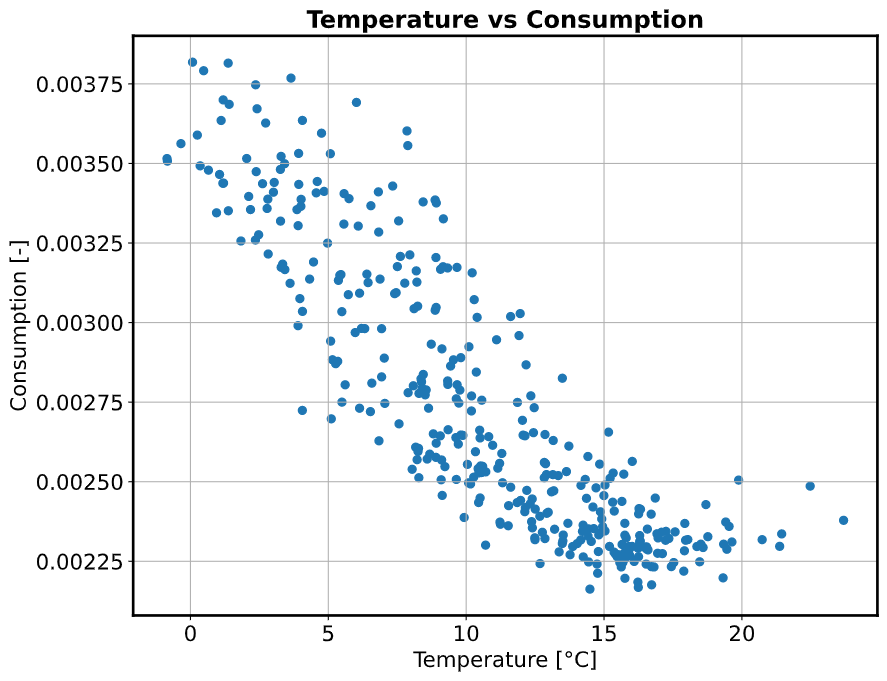
\includegraphics[width=0.8\textwidth]{pearson.png}
	\caption{Relation between consumption and temperature.}
	\label{fig:pearson}
\end{figure}

This figure shows the classic cone-shaped pattern of heteroscedasticity. On days when it is warm there is overall similar human behaviour in lowering the electricity consumption. However, on colder days the variation in consumption is higher. Because the assumptions of the Pearson correlation are not fulfilled, care should be taken with its output.\\

Applying the Pearson correlation on Figure \ref{fig:pearson} gives a correlation value of $ -0.85 $. This means there is a reasonable linearly decreasing relation.\\


\textbf{Spearman correlation}\\
Spearman correlation is a ``Rank correlation''. This means that the ordering of the consumption and temperature in a sample are each compared in their corresponding array of measurements.  When the ordering of both variables in a sample are similar, correlation is strong and positive. If the ordering is reversed, correlation is strong and negative. There is a perfect positive ordering if larger consumption always corresponds to a higher temperature. Notice that for a perfect ordering, no linear relation of the variables is necessary. The Spearman correlation coefficient is calculated using equation \ref{eq:pearson}, but takes into account the rank of a variable in all the measurements of this variable instead of the measurement value itself.\\

In order to use the spearman correlation data has to be ordinal, which means that it can be ordered. The spearman correlation gives information about the monotonicity relation between the variables. $ \rho = 1 $ corresponds to a monotonically increasing relation.\\

Applying the Spearman correlation  gives a correlation value of $ -0.87$, which means there is a reasonable negative monotonicity relation.\\

\textbf{Kendal correlation}
The ``Kendal correlation'' is also a rank based correlation. Here it is looked at the pairs of observation that are concordant, discordant or neither. A correlation coefficient close to one occurs when both variables have the same ranking and similar a coefficient close to minus one occurs when rankings in one variable are the reverse of the other. Equation \ref{eq:kendall} gives the equation to calculate the ``Kendal correlation coefficient''.

\begin{equation}\label{eq:kendall}
	\tau = \frac{n^+-n^-}{\sqrt{(n^++n^-+n^x)(n^++n^-+n^y)}}
\end{equation}
\begin{itemize}
	\item $ n^+ $ is the number of concordant pairs
	\item $ n^- $ is the number of discordant pairs
	\item $ n^x $ is the number of ties only in x
	\item $ n^y $ is the number of ties only in y
	\item concordant $\rightarrow $ $ (x_i > x_j ) $ and $ (y_i > y_j ) $ or $ (x_i < x_j ) $ and $ (y_i < y_j ) $
	\item discordant $\rightarrow $ $ (x_i > x_j ) $ and $ (y_i < y_j ) $ or $ (x_i < x_j ) $ and $ (y_i > y_j ) $
	\item neither $\rightarrow $ $ (x_i = x_j ) $ or $ (y_i = y_j ) $
	\item if both $ (x_i = x_j ) $ and $ (y_i = y_j ) $ $\rightarrow $ not included in either $ n^x $ or $ n^y $
\end{itemize}

Applying the Kendal correlation  gives a correlation value of $ -0.66$, which means there is a reasonable negative monotonicity relation.\\

% There is a clear dependency between temperature and electricity consumption, which means that electricity is used for heating.  


\subsection{Comparing weekdays with weekends}



\subsection{Impact of holidays}
% important that look at holidays in the UK. In paper \cite{Hoverstad2015} all the holydays are subsitued by the same day the next week and the previous week. It is possible to look at all the holidays, normalize them concerning temperature and try to get a seasonality model. 



\section{ARIMA}
% Idea is to use the simple ARIMA model as a base line forecasting model. 
% see datacamp and youtube Lola
% ARIMA assumes stationary data.
What is ARIMA. 
Assumptions of ARIMA...

\textbf{Stationarity}\\
 https://machinelearningmastery.com/remove-trends-seasonality-difference-transform-python/
When data is modelled it is assumed that the statistics of the data are consistent or stationary. This means the mean and standard deviation is not changing in time. However, because time series are often subdued to a trend or seasonality this assumption of stationarity is violated. In order to model not stationary observations by a stationary model as ARIMA, trends and seasonal effects should be removed. A way to check the stationarity of your observations, the ``Dicky-Fuller test'' can be used.
A way to remove non-stationarity is by using ``Difference Transform''. Here the trend and seasonality is subtracted from the observations leaving behind a stationary dataset.


\section{Conclusion}
The final section of the chapter gives an overview of the important results
of this chapter. This implies that the introductory chapter and the
concluding chapter don't need a conclusion.




%Please don't abuse enumerations: short enumerations shouldn't use
%``\verb|itemize|'' or ``\texttt{enumerate}'' environments.
%So \emph{never write}: 
%\begin{quote}
%	The Eiffel tower has three floors:
%	\begin{itemize}
%		\item the first one;
%		\item the second one;
%		\item the third one.
%	\end{itemize}
%\end{quote}
%But write:
%\begin{quote}
%	The Eiffel tower has three floors: the first one, the second one, and the
%	third one.
%\end{quote}

%%% Local Variables: 
%%% mode: latex
%%% TeX-master: "thesis"
%%% End: 
